\section{Business vocabulary flows out of software, and entrants do not carry it disproportionately}\label{sec:diffusion}

The spatial version of this question is answered: \citet{vonGraevenitz2022}
show that novel description tokens reach distant US locations more slowly
than near ones, in the \emph{Regional Studies} programme surveyed by
\citet{CastaldiMendonca2022}. The cross-industry version is open, and the
Nice class system supplies the partition.

For nine curated business-model phrases, Table~\ref{tab:transit} records
the first year each of four classes (software 009, tech services 042,
transport 039, advertising/retail 035; 2.32 million granted filings)
crosses a 1\% prevalence floor. Software- and tech-services-origin
phrases arrive in the physical-economy classes with lags of one to
thirteen years; the only counterexample in the set is on-demand, which
originates in transport. The 1\% floor is sensitive to class size, and
the asymmetry is a four-class result a 45-class build would test
properly.

\begin{table}[h]\centering\small
\caption{First year a theme reaches 1\% prevalence among granted filings,
by class. ``--'' = never clears the floor.}
\label{tab:transit}
\begin{tabular}{lrrrr}
\toprule
Theme & software & tech-svcs & transport & advert/retail \\
\midrule
as-a-service              & 2011 & \textbf{2009} & 2013 & 2012 \\
mobile-app                & 2010 & \textbf{2009} & 2012 & 2012 \\
cloud                     & 2012 & \textbf{2010} & 2011 & 2014 \\
streaming                 & \textbf{2008} & 2008 & 2013 & 2014 \\
artificial-intelligence   & 2017 & \textbf{2016} & 2018 & 2018 \\
augmented/virtual-reality & \textbf{2015} & 2016 & 2022 & 2022 \\
blockchain / crypto       & 2021 & \textbf{2018} & --   & 2022 \\
real-time                 & \textbf{2001} & 2003 & 2009 & 2014 \\
on-demand                 & 2017 & 2016 & \textbf{2014} & 2017 \\
\bottomrule
\end{tabular}
\end{table}

Unsupervised theme extraction corroborates the pattern without depending
on which phrases were picked. A detection-purpose latent Dirichlet allocation
(LDA) topic model ($T = 50$ on a
stratified 200{,}000-filing sample) yields recognizable business-model
components; for each (theme, class) cell crossing the 1\% floor with six
or more tracked years, Bass-model fits \citep{Bass1969} on 118 retained
cells give median innovation coefficient $p = 0.018$, median imitation
coefficient $q = 0.110$, and median $q/p \approx 6.5$, in the range
typically reported for consumer-product adoption. Tagging each
multi-class theme's origin class and counting directed origin-to-arrival
edges: software contributes 33 of 72 edges against 18 expected under
symmetry, and receives only 10. The asymmetry reproduces under
independently-fitted non-negative matrix factorization (NMF) on the same
sample; both are bag-of-words
factorizations, so the robustness is within-paradigm.

Entrants carry the canonically new themes, but no more often than they
carry anything else. The 50
earliest carriers per theme are 73.7\% entrants on average --- but the
corpus's year-matched debut baseline is 76.4\%, so the theme-carrier
excess is $-2.7$pp and 28 of 50 themes sit \emph{below} baseline.
The themes leaning incumbent include environmental/sustainability, natural
gas and petroleum, artificial intelligence, and cloud computing. So the arrival of new vocabulary is not an entrant
phenomenon in the way the Schumpeterian reading would predict
\citep{Schumpeter1942}.

The AI era has so far compounded rather than erupted, though the most recent
data test that reading rather than confirming it. Dating each era from
the first year its terms appear in at least 0.4\% of filings in the two
classes --- 1994 for the internet, 2015 for AI, in both cases the year
before the share at least doubled --- the two track closely through year three, then
diverge: internet vocabulary tripled between years four and six to 23\% of
filings in 2000, while AI vocabulary reaches 12.9\% at year nine, roughly
where the internet stood at year five (Figure~\ref{fig:era}). The last two
observed years are the steepest in the series --- prevalence rises about
14\% a year to 2021, then 50\% between 2022 and 2023 and 26\% into 2024,
following the release of consumer chatbots. That is an acceleration rather
than a discontinuity, since per-year corpus turbulence shows no AI-era
deviation through 2024, but it runs in the direction the eruption reading
predicts. The comparison is sensitive to the era-start alignment, and the
falsifiable marker is close to binding: if AI follows the internet's path
with a lag, its prevalence should triple within roughly three years of the
2024 edge and the entrant share of its carriers should rise above baseline.

\begin{figure}[h]\centering
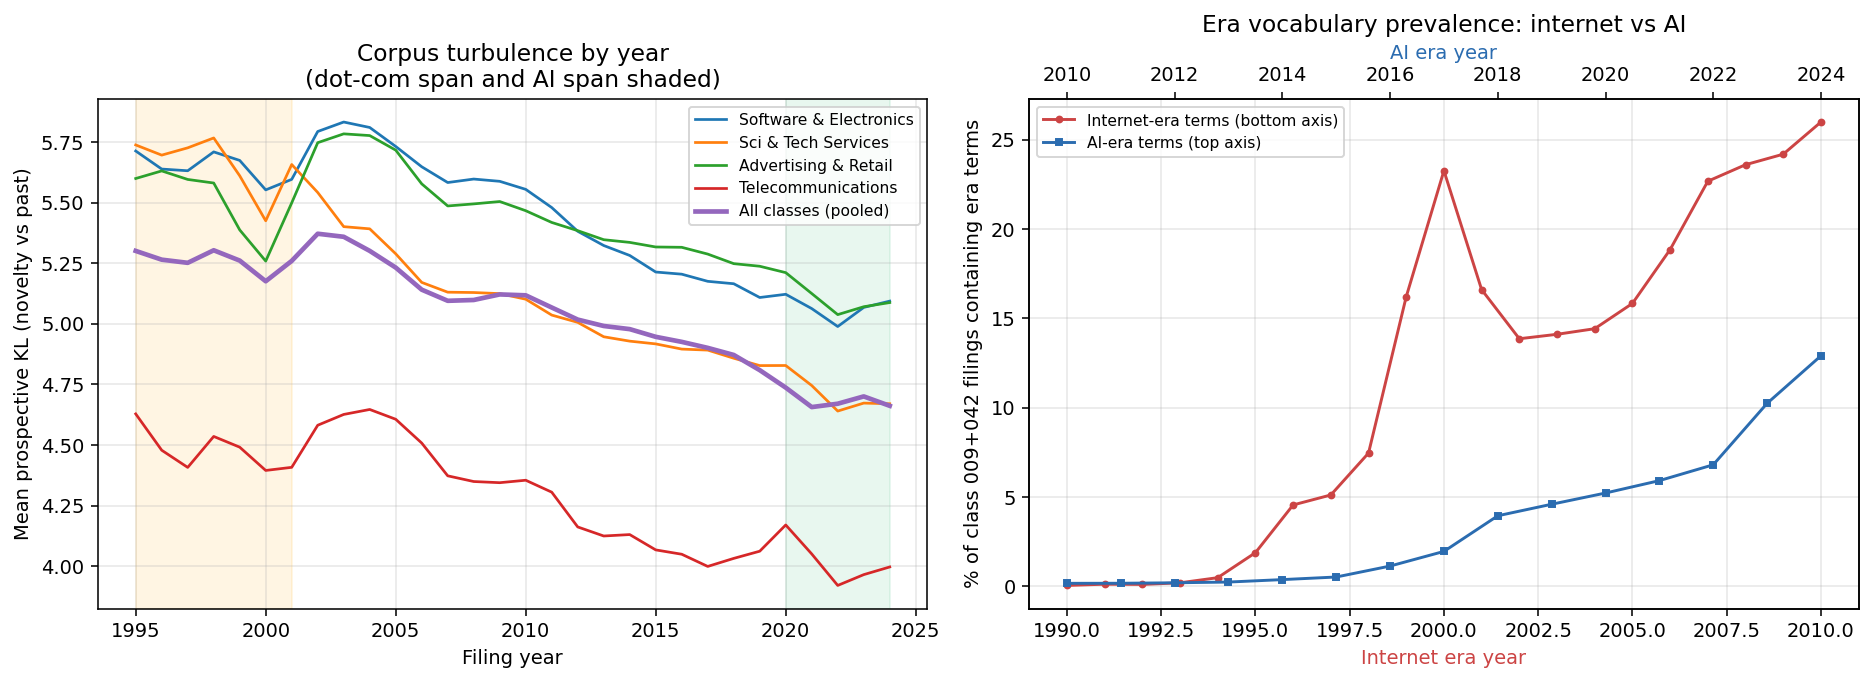
\includegraphics[width=\textwidth]{results/era_turbulence.png}
\caption{\emph{Left:} per-year mean past-facing surprise by class and pooled,
1995--2024, with the dot-com and AI spans shaded. \emph{Right:} share of
class 009+042 filings whose goods/services text contains internet-era terms
(internet, website, online, world wide web) or AI-era terms (artificial
intelligence, machine learning, generative, neural network, chatbot, and
kin), plotted in era years. Year 0 of each era is the first calendar year
in which its terms reached 0.4\% of the two classes' filings: 1994 for the
internet, 2015 for AI. The two calendar axes share one scale, one year per
unit of width; the AI series ends at 2024, nine years in, where the record
ends, and has not yet run the internet's sixteen.}
\label{fig:era}
\end{figure}

